\documentclass[12pt,a4paper]{article}

\usepackage{german}      % Deutsche TeX-Eigenheiten
%\usepackage{isolatin1}   % Eingabekodierung mit Umlauten...

\usepackage{makeidx}
\makeindex            % damit eine Indexdatei angelegt wird

\usepackage{graphicx}

\usepackage{amsmath}  % allgemeine Mathe-Erweiterungen
\usepackage{amssymb}  % Symbole und Schriftarten
\usepackage{amsthm}   % erweiterte Theorem-Umgebungen

\usepackage{mathrsfs}  % gibt den Befehl "\mathscr{}" f�r sch�ne

\begin{document}

\section{Seminar 1 - L'Hospital + Taylorsche Formel}
\subsection{L'Hospital}
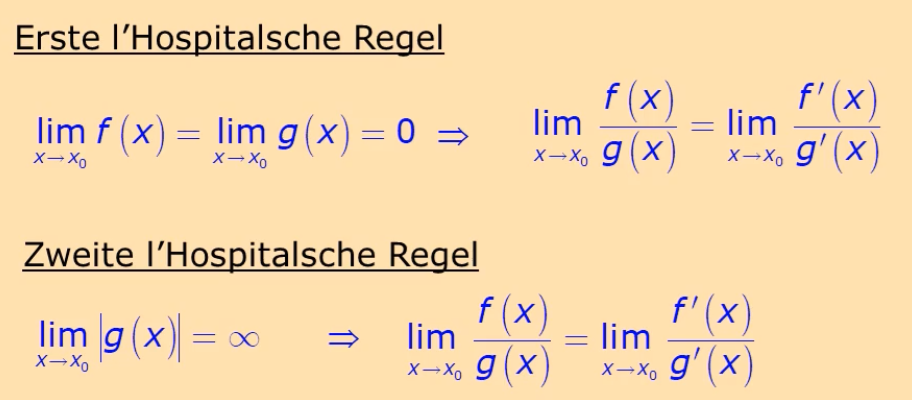
\includegraphics[width=0.8\textwidth]{BIlder/S1/1.png}\\
Die Erste Untersucht 0/0\\
Die Zweite setzt vorraus, dass g gegen +/- Unendlich geht\\
\subsubsection{1. Aufgabe}

\includegraphics[width=0.8\textwidth]{BIlder/S1/2.png}\\
Werkzeug:\\
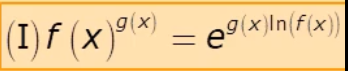
\includegraphics[width=0.3\textwidth]{BIlder/S1/3.png}\\
Damit erstmal umformulieren:\\
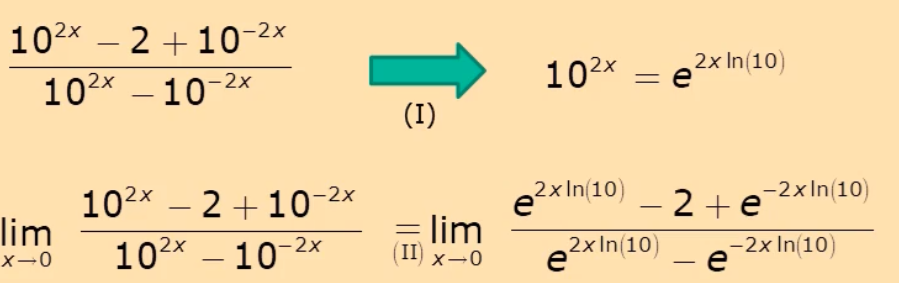
\includegraphics[width=0.8\textwidth]{BIlder/S1/4.png}\\
Typ 0/0\\
\newpage
Nächstes Werkzeug:\\
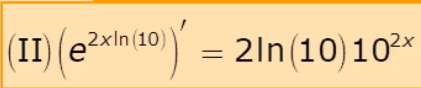
\includegraphics[width=0.3\textwidth]{BIlder/S1/5.png}\\
Daraus ergibt sich:\\
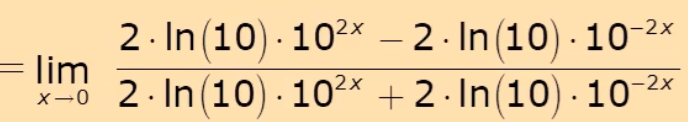
\includegraphics[width=0.6\textwidth]{BIlder/S1/6.png} = 0\\
\subsubsection{2. Aufgabe}
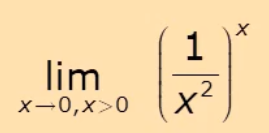
\includegraphics[width=0.2\textwidth]{BIlder/S1/7.png}\\
1. Typ bestimmten: Unendlich(hoch)0\\
Nicht für die Regeln 1/2 geeignet\\
Werkzeug:\\
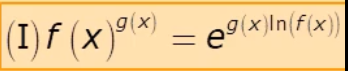
\includegraphics[width=0.3\textwidth]{BIlder/S1/3.png}\\
Daraus folgt:
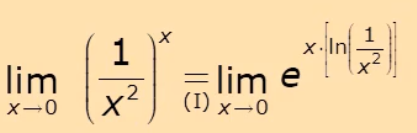
\includegraphics[width=0.3\textwidth]{BIlder/S1/8.png}\\
Weiter Umstellen mit Multiplikationstheorem:
\includegraphics[width=0.3\textwidth]{BIlder/S1/10.png}\\\\
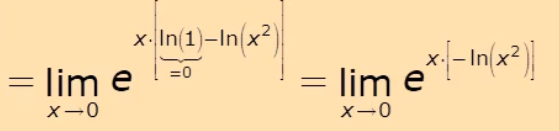
\includegraphics[width=0.5\textwidth]{BIlder/S1/9.png}\\
Weiter Umstellen, da e-fkt stetig:\\
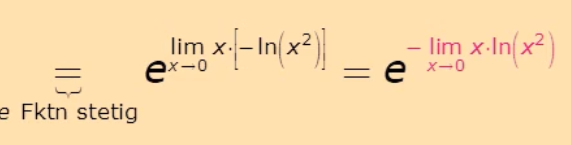
\includegraphics[width=0.5\textwidth]{BIlder/S1/11.png}\\
Typbestimmung... wie verhält sich der logarithmus ?\\
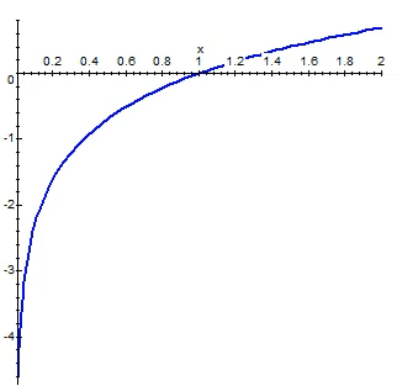
\includegraphics[width=0.2\textwidth]{BIlder/S1/12.png}\\
Typ - Unendlich * 0\\
\newpage
Werkzeug:\\
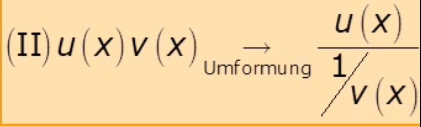
\includegraphics[width=0.2\textwidth]{BIlder/S1/13.png}\\
Daraus ergibt sich:
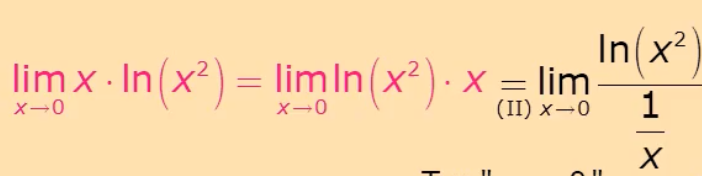
\includegraphics[width=0.4\textwidth]{BIlder/S1/14.png}\\
Was ist, wenn x gegen 0 geht ? = -Unendlich/Unendlich\\
Anwendung 2. L'Hospital regel:
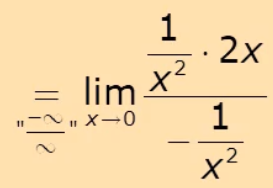
\includegraphics[width=0.2\textwidth]{BIlder/S1/15.png}\\
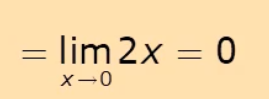
\includegraphics[width=0.2\textwidth]{BIlder/S1/16.png}\\
Jetzt wieder zusammensetzten:
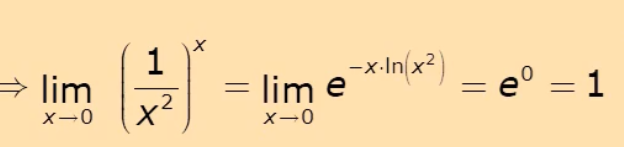
\includegraphics[width=0.5\textwidth]{BIlder/S1/17.png}\\
\end{document} 